\title{Neural Networks - Final Report: Learning Vector Quantization}
\author{Ryan Spangler}
\date{\today}

\documentclass[12pt]{article}

\usepackage{commath}
\usepackage{graphicx}
\usepackage{listings}
\usepackage{amsfonts}

% python highlighting ----------
\usepackage{color}
\usepackage{listings}
\usepackage{textcomp}
\usepackage{setspace}
%\usepackage{palatino}

\renewcommand{\lstlistlistingname}{Code Listings}
\renewcommand{\lstlistingname}{Code Listing}
\definecolor{gray}{gray}{0.6}
\definecolor{green}{rgb}{0.1,0.6,0.3}
\definecolor{orange}{rgb}{0.9,0.7,0.1}
\definecolor{blue}{rgb}{0,0.6,0.8}

\lstnewenvironment{python}[1][]{
\lstset{
language=python,
basicstyle=\ttfamily\footnotesize\setstretch{1},
stringstyle=\color{red},
showstringspaces=false,
alsoletter={1234567890},
otherkeywords={\ , \}, \{},
keywordstyle=\color{blue},
emph={access,and,break,class,continue,def,del,elif,else,%
except,exec,finally,for,from,global,if,import,in,is,%
lambda,not,or,pass,print,raise,return,try,while},
emphstyle=\color{gray}\bfseries,
emph={[2]True, False, None, self},
emphstyle=[2]\color{orange},
emph={[3]from, import, as},
emphstyle=[3]\color{blue},
upquote=true,
morecomment=[s]{"""}{"""},
commentstyle=\color{gray}\slshape,
emph={[4]1, 2, 3, 4, 5, 6, 7, 8, 9, 0},
emphstyle=[4]\color{blue},
literate=*{:}{{\textcolor{blue}:}}{1}%
	{=}{{\textcolor{blue}=}}{1}%
	{-}{{\textcolor{blue}-}}{1}%
	{+}{{\textcolor{blue}+}}{1}%
	{*}{{\textcolor{blue}*}}{1}%
	{!}{{\textcolor{blue}!}}{1}%
	{(}{{\textcolor{blue}(}}{1}%
	{)}{{\textcolor{blue})}}{1}%
	{[}{{\textcolor{blue}[}}{1}%
	{]}{{\textcolor{blue}]}}{1}%
	{<}{{\textcolor{blue}<}}{1}%
	{>}{{\textcolor{blue}>}}{1},%
    frame=fullbox, rulesepcolor=\color{gray},#1
%framexleftmargin=1mm, framextopmargin=1mm, frame=shadowbox, rulesepcolor=\color{blue},#1
}}{}

\setcounter{secnumdepth}{0}

\begin{document}
\maketitle

\section{Abstract}

This paper explores the Linear Vector Quantization (LVQ) neural network paradigm and its application to a real world problem.  Given a set of training data about land use, this experiment proceeds to train the network to optimal performance, then progressively remove features until only the essential features remain.  Using this subset of features, the network is able to be trained to high optimality.  

\section{Introdution/Background on LVQ}

The LVQ is a supervised training algorithm that relies on competition between its PEs to attain a classification of inputs according to a scheme it discovers through training.  During training the incoming vectors are compared against the vectors represented by each PE.  The closest one is considered the ``winner'' and its output is transmitted to the next layer to determine which class the input vector belongs to.  If it is the correct class, the PE is moved closer to the input vector, and if not it is moved away (this is known as ``repulsion'').  After the network has been trained, it performs classification according to the same principles, only the vectors for each PE are no longer moved.  Each pass through the network at this point represents a classification of the vector to one of a certain number of classes, determined by the number of output elements chosen before training.  

The overall effect of the LVQ is ``as if'' the network is optimized to classify its set of presented data according to the classes associated with them, regardless of the nature of the data and without having to have any specific knowledge about the data outside of what classes each training vector belongs to. 

\section{Problem Statement}

The problem for this project is, given the training data set of 52 features and using the LVQ neural network paradigm, discover the smallest subset of features that enables the network to correctly classify the data above 90\% of the time.  It is claimed that 9 features is sufficient for the network to achieve these results, and that even smaller subsets are possible.  My task is to find this minimal subset.

\section{Experimental Process}

The first step was to train an LVQ network with the full set of 52 features.  This was done by creating an LVQ network in NeuralWorks (NW) from the InstaNet menu.  The parameters were as follows:

\begin{center}
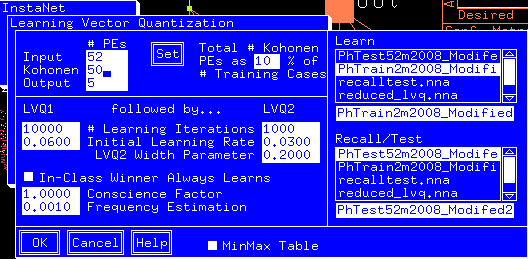
\includegraphics[scale=0.7]{parameters52features.png}
\end{center}

The main notable parameter in this table is the number of Kohonen PE's, which I chose to be 50.  In the documentation of the LVQ it says there must be the same number of competitive layer PE's for each output, so I chose for this experiment to have 10 PE for each of the 5 outputs.  I was suspicious of this however, so I tried again with 15 to see if this made any difference in the results.  

The parameters for this experiment are given below:





The weight matrix can be viewed in two ways.  In the first, and how the network is trained, the value for each feature is applied to each PE.  These features form an instar, and the PE receives one input from each feature, multiplied by the corresponding weight for that feature to that PE.  So in training, the weight matrix is spliced along the rows to make vectors of distinct feature weights, each of which is then multiplied by the input vector to get the input to each PE.

The other way to look at the weight matrix is to splice it along its columns into vectors of values adopted by a single feature across all presentations.  These vectors supply a complementary perspective, where each of the features is portrayed independently of their relationship to other features.  

The discovery of the critical 5 features was due to a fortuitous insight.  Since all of the data from the training set was in the positive range, training of salient features (which involved moving the vector for the PE towards the input vector upon winning the competition) would on average increase the weight vector for that feature, if the feature contributed to correctly classifying the input.  Therefore, when I subtract the weight vectors of an untrained network from those of its weights after training, the features corresponding to weight vectors with a positive overall change (sum of elements) were the ones that were critical for the correct classification of the input data.    

Performing this analysis on the data I revealed five features whose total sum of the change in feature-related weights was positive, the rest were all negative.  Reducing the feature set to only these five, I started from a fresh network with only five inputs and trained it from this limited set.  

\begin{center}
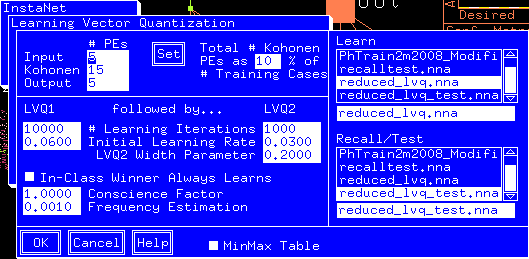
\includegraphics[scale=0.7]{parameters5features.png}
\end{center}

To ensure that this was indeed the correct set of 5 features I took a control group of 5 features that all showed negative total weight modification (actually, simply the first 5 features from the training set) to compare the performance against the 5 with positive weight modification.  For this run, all parameters were identical except the training and testing data sets:

\begin{center}
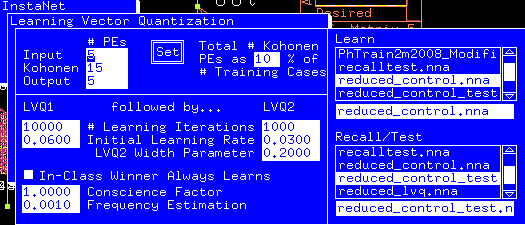
\includegraphics[scale=0.7]{parameters5control.png}
\end{center}

I found these sufficient steps to uncover the critical 5 features necessary to correctly classify the test data with a performance greater than 90\%.  

\subsection{Results}

Numbering the 52 features from 0-51 in the order given in the test data, the critical 5 features that attained almost 92\% classification accuracy were

\begin{itemize}
\item 13
\item 44
\item 45
\item 46
\item 49
\end{itemize}

The other features were more or less irrelevant, or at best redundant.  The presence of all the other features combined contributed only a 1-2\% increase in classification performance.

\section{Conclusion}

Ultimately, finding the ideal subset of 5 features that could be used to adequately classify the vectors from the test set was not difficult, as their relative applicability was encoded in the values of the weights from each input to the competitive PEs.  The network naturally excluded features that did not contribute to the classification through inhibitory weight modifications.  Only the features that actually correlated to the desired classification scheme were encouraged through weight increases, the others were effectively rendered irrelevant.  

\end{document}  

